%----------------------------------------------------------------------
\documentclass[a4paper,12pt]{book}
\usepackage[utf8]{inputenc}
%----------------------------------------------------------------------

% Document variables
\newcommand{\doctitle}{Computer methods for astrodynamics}
\newcommand{\docsubtitle}{Includes examples with poliastro software}
\newcommand{\authorname}{Jorge Martínez}
\newcommand{\authordepartment}{Open Source Community}
\newcommand{\authordepartmenturl}{}
\newcommand{\docversion}{First}

% Macros
% Load packages
\usepackage{graphicx,amsmath,amsfonts,amssymb,color,
dcolumn,siunitx,longtable,bm,paralist,setspace,rotating,array,fix-cm,
multirow,multicol,hhline,enumitem,cancel,tikz,listings,ifthen,mathabx,
framed,caption,pdfpages,eurosym}

% Fourier font is beautiful
\let\widering\relax
\usepackage{fourier}

\usepackage[a4paper]{geometry} 
\usepackage[super,ref]{cite}
\usepackage[yearmonthsep={},monthdaysep={}]{datetime2}

% hyperref and associated packages
\usepackage[unicode=true,bookmarks=true,bookmarksopen=false,
	bookmarksopenlevel=1,pdfborder={0 0 0},backref=false,
	colorlinks=true,allcolors=magenta,pdfstartview=Fit,
	pdfcenterwindow=true,pdfdisplaydoctitle=true,
	pdfpagelayout=OneColumn,linktocpage=true]{hyperref}
\hypersetup{pdfauthor={\authorname},pdftitle={\doctitle\ -- \docsubtitle},
pdfproducer={\authordepartment}}

% fancyhdr
\newgeometry{left=2.8cm,right=2.8cm,bottom=3cm,top=3cm}
\usepackage{fancyhdr}
\pagestyle{fancy}
\renewcommand{\headrulewidth}{0.4pt}
\renewcommand{\footrulewidth}{0.4pt}
\fancyhead[L]{\nouppercase{\leftmark}}
\fancyhead[C]{}
\fancyhead[R]{\doctitle}
\fancyfoot[L]{\thepage}
\fancyfoot[C]{\authordepartment}
\fancyfoot[R]{Version \docversion}  

% maths
\newcommand{\const}{\text{const}} 
\newcommand{\etal}{{\it et al. }}
\newcommand{\oone}{\mathcal{O}(1)} 
\newcommand{\paren}[1]{\left( #1 \right)} 
\newcommand{\brckt}[1]{\left[ #1 \right]} 
\newcommand{\pd}{\partial} 
\newcommand{\pr}{^\prime}
\newcommand{\dd}{\mathrm{d}}

% text
\newenvironment{inlist} % Use inlist for inline lists with roman numerals  
	{\begin{inparaenum}[(\itshape i\/\upshape )]} {\end{inparaenum}}
\newcommand{\mycite}[1]{[\citen{#1}]}

% multicol 
\setlength\columnseprule{.4pt}
\raggedcolumns

% itemize item vertical separation distance
\setitemize{noitemsep}

% number figures, tables and equations within sections
\numberwithin{equation}{section}
\numberwithin{figure}{section}

% fancy chapters
\usepackage{titlesec}
\titleformat{\chapter}[display]
{\bfseries\Large}
{\filright\MakeUppercase{\chaptertitlename} \Huge\thechapter}
{2ex}
{\titlerule\vspace{2ex}\filleft}
[\vspace{2ex}\titlerule]







% theorems box
\usepackage{cleveref}
\usepackage[most]{tcolorbox}
\definecolor{poliastro_blue}{rgb}{0.0, 0.5, 1.0}

\newtcbtheorem{Definition}{Definition}{
	enhanced,
	sharp corners,
	attach boxed title to top left={
		yshifttext=-1mm
	},
	colback=radian_blue!25!,
	colframe=poliastro_blue!75!black,
	fonttitle=\bfseries,
	boxed title style={
		sharp corners,
		size=small,
		colback=blue!75!black,
		colframe=blue!75!black,
	} 
}{thm}


%----------------------------------------------------------------------
\begin{document}
%----------------------------------------------------------------------

% Title page
% Title page 
% Must be inputted within \begin{document} \end{document}. 
% Requires mariomacros.tex and \doctitle, \docsubtitle, \authorname,
% \authordepartment

%----------------------------------------------------------------------
\pagenumbering{gobble} % removes page numbering, and pauses it

\begin{titlepage}
\newgeometry{left=1cm,right=1cm,bottom=1cm,top=1cm}
\clearpage

% Background color for the cover
\definecolor{radianBlue}{rgb}{0.0, 0.5, 1.0}
\definecolor{darktan}{rgb}{0.57, 0.51, 0.32}
\definecolor{mediumpersianblue}{rgb}{0.0, 0.4, 0.65}
\pagecolor{mediumpersianblue!50!}

\thispagestyle{empty}
\vspace*{\fill}

\begin{center} 
{\fontsize{60pt}{70pt}\selectfont \doctitle \par} 
\vspace{1cm}

\begin{figure}[h]
	\centering
	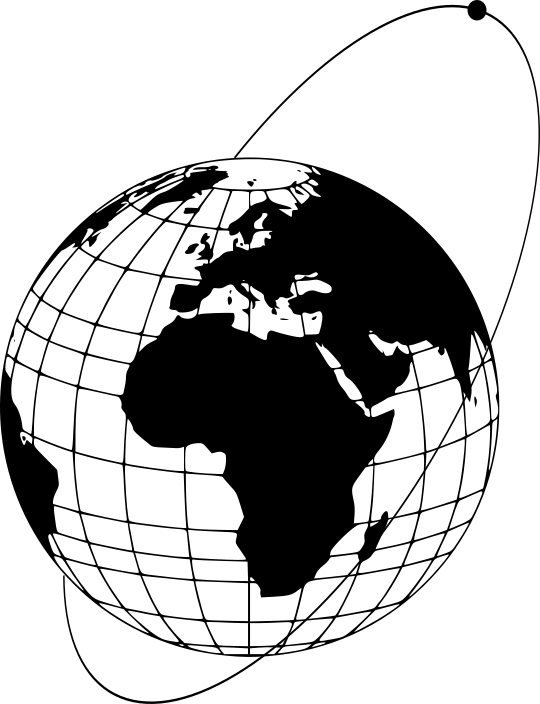
\includegraphics[scale=0.75]{figs/cover.png}
\end{figure}
\vspace{1cm}
{\Huge \sc \docsubtitle} 
\\[2cm]
{\huge \authorname}
\\[1cm]
{\Large \docversion \hspace{0.05cm} Edition}
%\\[2cm]
%{\Large \sc %\href{\authordepartmenturl}{\authordepartment}} 
\end{center}
\vspace*{\fill}
\end{titlepage} 
%----------------------------------------------------------------------

%---------------------------------------------------------------------- 
\newgeometry{left=2.8cm,right=2.8cm,bottom=3cm,top=3cm}
\pagenumbering{arabic} % restores page numering and resumes it
\thispagestyle{empty}
%\newpage
\definecolor{mediumpersianblue}{rgb}{0.0, 0.4, 0.65}
\pagecolor{mediumpersianblue!25!}

\newpage
 \hbox{}
\newpage
%----------------------------------------------------------------------


% Preface and table of contents
%----------------------------------------------------------------------
\section*{Preface}
%----------------------------------------------------------------------

This book tries to describe in detail all the principles for astrodynamics, orbital mechanics and orbit determination. Reader will also find non common topics such us time-scales, reference frames and low-thrust maneuvers, for example. My intention writing this book is not only to have a reference manual on astrodynamics but also an open-source book on the topic, so anyone can contribute and add more information, chapters, references or algorithms.\\

Some errata may appear along this book, although intention is always good. If found, please send me an email to \href{mailto:ingenierodeaviones@gmail.com}{ingenierodeaviones@gmail.com} or just open an issue in the official GitHub repository at \href{https://github.com/jorgepiloto/astrobook}{https://github.com/jorgepiloto/astrobook}. You can also correct by yourself the errata and open a pull request so it can be corrected in future versions.\\

Finally, I want to thank all open-source community. No matter if you contribute to scientific, engineering or web projects, sharing knowledge will guide humanity towards a real free world. For that reason this book has been developed using only open-source tools such us \LaTeX, Inkscape and Python.
\tableofcontents

% Chapters
%----------------------------------------------------------------------
\chapter[A brief introduction to astrodynamics]{A brief introduction to astrodynamics}
%----------------------------------------------------------------------
 
We usually refer to celestial mechanics, astrodynamics, orbital dynamics, attitude dynamics or astronomy as the same thing. However it is important to make clear that these concepts differ from each other and we should properly understand what we refer to when talking about each one. Let us start this chapter by defining them in detail:

\vspace{0.25cm}
\begin{Definition*}{}
	\textbf{Celestial mechanics} is the scientific study of celestial body dynamics.
\end{Definition*}
\vspace{0.25cm}

\vspace{0.25cm}
\begin{Definition*}{}
	\textbf{Orbital dynamics} is the scientific study of the motion of small orbiting bodies.
\end{Definition*}
\vspace{0.25cm}

\vspace{0.25cm}
\begin{Definition*}{}
	\textbf{Attitude dynamics} is the scientific study of the relative position and orientation of bodies in space.
\end{Definition*}
\vspace{0.25cm}

\vspace{0.25cm}
\begin{Definition*}{}
	\textbf{Astronomy} is  the scientific study of matter and phenomena in the universe, especially in outer space, including the positions, dimensions, distribution, motion, composition, energy, and evolution of celestial objects.
\end{Definition*}
\vspace{0.25cm}

\begin{Definition*}{}
	\textbf{Astrodynamics} is the branch of astronomy that studies the motion of celestial and man-made bodies in space subjected to both natural and artificial perturbations.
\end{Definition*}
\vspace{0.25cm}

\section{The Solar System models}

When first human beings started to look at the stars, they tried to explain 

\begin{figure}[h]
	\centering
	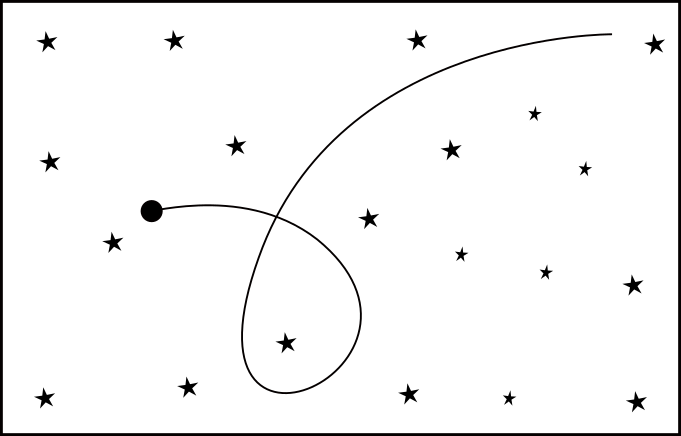
\includegraphics[scale=0.75]{figs/sky_path.png}
	\caption{Apparent path of a celestial body}
\end{figure}


\newpage
\section{Solar System bodies}

\begin{figure}[h]
	\centering
	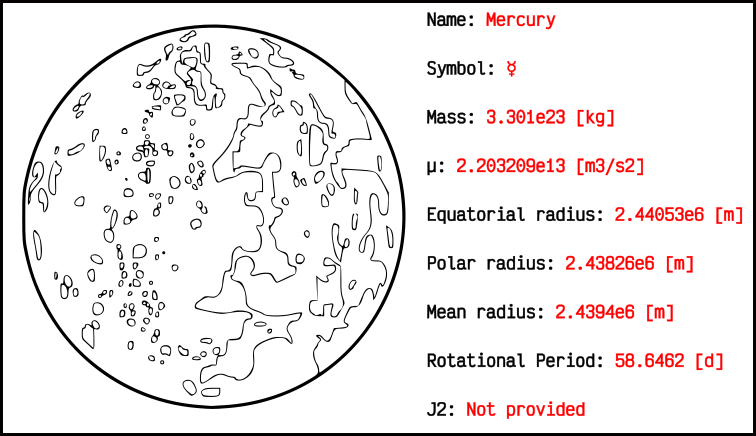
\includegraphics[scale=0.85]{figs/bodies/mercury.png}
	\caption{Mercury data}
\end{figure}

%Bibliography
\nocite{*}
\bibliographystyle{plain}
\bibliography{bibliography}

%----------------------------------------------------------------------
\end{document}
%----------------------------------------------------------------------
